%%%%%%%%%%%%%%%%%%%%%%%%%%%%%%%%%%%%%%%%%%%%%%%%%%%%%%%%%%%%%%%
%
% Welcome to Overleaf --- just edit your LaTeX on the left,
% and we'll compile it for you on the right. If you open the
% 'Share' menu, you can invite other users to edit at the same
% time. See www.overleaf.com/learn for more info. Enjoy!
%
%%%%%%%%%%%%%%%%%%%%%%%%%%%%%%%%%%%%%%%%%%%%%%%%%%%%%%%%%%%%%%%



% Inbuilt themes in beamer
\documentclass{beamer}

% Theme choice:
\usetheme{CambridgeUS}
\setbeamertemplate{caption}[numbered]{}

\usepackage{enumitem}
\usepackage{tfrupee}
\usepackage{amsmath}
\usepackage{amssymb}
\usepackage{gensymb}
\usepackage{graphicx}
\usepackage{txfonts}

\def\inputGnumericTable{}

\usepackage[latin1]{inputenc}                                 
\usepackage{color}                                            
\usepackage{array}                                            
\usepackage{longtable}                                        
\usepackage{calc}                                             
\usepackage{multirow}                                         
\usepackage{hhline}                                           
\usepackage{ifthen}
\usepackage{caption} 
\captionsetup[table]{skip=3pt}  
\providecommand{\pr}[1]{\ensuremath{\Pr\left(#1\right)}}
\providecommand{\brak}[1]{\ensuremath{\left(#1\right)}}
\providecommand{\cbrak}[1]{\ensuremath{\left\{#1\right\}}}
\renewcommand{\thefigure}{\arabic{table}}
\renewcommand{\thetable}{\arabic{table}}
\makeatletter
\@addtoreset{figure}{problem}
\makeatother
\let\StandardTheFigure\thefigure
\let\vec\mathbf
\renewcommand{\thefigure}{\theproblem}
\def\putbox#1#2#3{\makebox[0in][l]{\makebox[#1][l]{}\raisebox{\baselineskip}[0in][0in]{\raisebox{#2}[0in][0in]{#3}}}}
     \def\rightbox#1{\makebox[0in][r]{#1}}
     \def\centbox#1{\makebox[0in]{#1}}
     \def\topbox#1{\raisebox{-\baselineskip}[0in][0in]{#1}}
     \def\midbox#1{\raisebox{-0.5\baselineskip}[0in][0in]{#1}} 
\renewcommand{\thefigure}{\theenumi}   


% Title page details: 
\title{AI1110 : Probability and Random Variables}
\subtitle{Assignment 5} 
\author{Mannem Charan(AI21BTECH11019)}
\date{\today}


\begin{document}
% Title page frame
\begin{frame}
    \titlepage 
\end{frame}


% Outline frame
\begin{frame}{Outline}
    \tableofcontents
\end{frame}


% Lists frame
\section{Question}
\begin{frame}{Question}
Prove and generalise the following identity
       \begin{equation}
          \begin{split}
              \pr{A+B+C} = \pr{A} + \pr{B} + \pr{C}\\ 
                                          - \pr{AB} -\pr{BC} \\
                                          -\pr{CA} + \pr{ABC}
         \end{split}
        \end{equation}
\end{frame}

\section{Solution}
\subsection{Proof}
  \begin{frame}{Solution:Proof}
       We will use the following identity,
              \begin{align}
                 \pr{A+B} &= \pr{A} +\pr{B} - \pr{AB}\label{eq:2}
              \end{align}
        Now from \eqref{eq:2}
              \begin{align}
                \pr{A + \brak{B + C}} &= \pr{A} + \pr{B+C}\label{eq:3}\\
                                                 & - \pr{A\brak{B+C}}\nonumber \\
                \pr{B+C} &= \pr{B} + \pr{C} - \pr{BC}\label{eq:4}\\
                \pr{A\brak{B+C}} &= \pr{AB + AC}\\
                                           & = \pr{AB} +\pr{AC}\\
                                            & -\pr{ABAC} \nonumber\\
                                           &= \pr{AB} +\pr{AC}\label{eq:7} \\ 
                                           &-\pr{ABC} \nonumber
               \end{align}
              \end{frame}
             \begin{frame}
           Substitute \eqref{eq:4} and \eqref{eq:7} in \eqref{eq:3}, we get
         \begin{equation}
           \begin{split}
              \pr{A+B+C} = \pr{A} + \pr{B} + \pr{C}\label{eq:9} \\  
                                                           - \pr{AB}  -\pr{BC}-\pr{CA} + \pr{ABC}
            \end{split}
        \end{equation}
         Now using induction, we can show similarly that,
             \begin{equation}
               \begin{split}
              \pr{A1+...+An} = \pr{A1} + ..... +\pr{An}\\
                                                   -\pr{A1A2}-... -\pr{An-1An}\\
                                            + ... \brak{-1}^{n-1}\pr{A1A2....An}
              \end{split}
             \end{equation}
           \end{frame}
   \subsection{Derivation}
        \begin{frame}{Solution:Derivation}
           We will derive \eqref{eq:2} using Boolean Algebra.For any two events A,B  
              \begin{align}
                    A.1 &= A\brak{B + B'}\\
                          &= AB + AB'\\
                    \pr{A} &= \pr{AB + AB'}\\
                               &= \pr{AB} + \pr{AB'} 
                  \end{align} 
          Since AB and AB' are mutually disjoint sets.\\ Now,
                   \begin{align}
                     A + B &= A\brak{B+B'} + B\brak{A+A'}\\
                              &= \brak{AB + BA} + BA' + B'A\\
                              &= AB + A'B + B'A\\
                              & = A + A'B
                    \end{align}
             \end{frame}
             \begin{frame}
            Now,
                 \begin{align}
                   \pr{A+B} &= \pr{A + A'B}
                 \end{align}
               Since both events are mutually disjoint.
                  \begin{align}
                   \pr{A+B}  & = \pr{A} + \pr{A'B}\\
                                  & = \pr{A} + \pr{B} - \pr{AB}
                  \end{align}
             \end{frame}
     \section{Verification}
       \begin{frame}{Verification}
          \begin{figure}[h!]
               \centering
               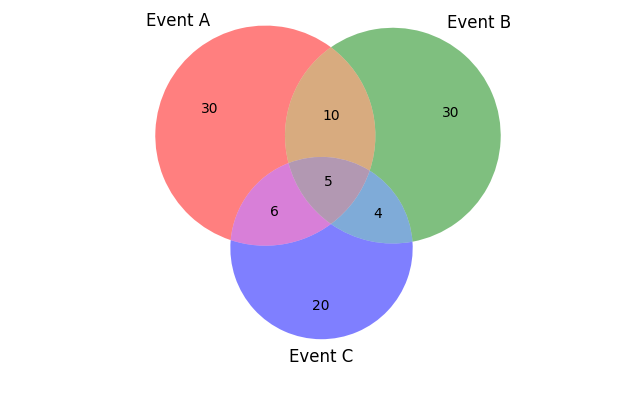
\includegraphics[width=\columnwidth]{venn_diagram.png}
               \caption{ Figure generated by python}
               \label{Figure 1}
             \end{figure}
           \end{frame}
         \begin{frame}
            The python code \texttt{./codes/verify.py} is used to verifiy the equation \eqref{eq:9} using above python generated figure.The ouput of code is shown below,
            \begin{figure}[h!]
              \centering
              
\includegraphics[width=\columnwidth]{output.png}
              \caption{}
             \end{figure}
              \end{frame}
      \end{document}